\section{Failure Taxonomy}
\label{sec:taxonomy}

Before attempting to repair agent failures, we must first diagnose \emph{what} fails and \emph{why}. We define a five-class failure taxonomy by analyzing failure cases from the Base condition (see \ref{sec:exp:cases}) across PinchBench (23 tasks) and AgentBench-OpenClaw (40 tasks). This taxonomy serves as the structural backbone of our repair study: we use it to define per-category repair rates (Eq~\ref{eq:crr}), to stratify our SFT data construction (\S\ref{sec:sft:data}), and to guide the design of training-free recipes (\S\ref{sec:recipes}).

% ------------------------------------------------------------
%  4.1  Taxonomy Definitions
% ------------------------------------------------------------

\subsection{Taxonomy Definitions}
\label{sec:taxonomy:definitions}

Each failure category has a precise operational definition, a set of diagnostic criteria, and a list of candidate repair strategies.

\bigskip
\noindent\textbf{A. Task Understanding / Planning Drift.}
\Category{A}

\textit{Definition:} The agent fails to correctly interpret the task requirements, constraints, or goal, or gradually drifts away from the core objective during multi-step execution.

\textit{Diagnostic criteria:} The agent's final answer or approach is misaligned with the task intent; evidence includes missing key constraints, pursuing a tangentially related subgoal, or producing an answer that addresses a different question than asked.

\textit{Example evidence:} For a medical question asking for differential diagnosis, the agent investigates only one disease; for a multi-hop QA question, the agent stops after finding one piece of evidence without checking whether additional hops are needed.

\textit{Candidate repairs:} Plan-first prompting, explicit subgoal tracking, periodic replanning, planner-executor role split.

\bigskip
\noindent\textbf{B. Tool / Environment Grounding Failure.}
\Category{B}

\textit{Definition:} The agent correctly understands \emph{what} it wants to do but fails to correctly map the intent to the correct tool, tool parameters, file path, or output format required by the execution environment.

\textit{Diagnostic criteria:} The agent calls the wrong tool, passes malformed arguments, uses an incorrect file path or URL, or produces output in a format incompatible with the tool's requirements. The failure occurs at the tool-call level, not the reasoning level.

\textit{Example evidence:} Calling \texttt{search\_engine} with a malformed query, accessing a file at the wrong path, or invoking \texttt{python\_exec} without required dependencies.

\textit{Candidate repairs:} Environment readiness checks, tool schema grounding, retry with error diagnosis, execution preflight checks.

\bigskip
\noindent\textbf{C. Memory / State Management Failure.}
\Category{C}

\textit{Definition:} The agent fails to stably maintain task context, intermediate facts, completed steps, generated artifacts, or prior search results across the interaction history.

\textit{Diagnostic criteria:} Evidence of repeated labor (re-searching the same query), lost intermediate conclusions, file or path confusion, or critical context being overwritten by subsequent turns. This failure is distinct from planning drift (category A) because the agent's plan is correct but its state tracking breaks down.

\textit{Example evidence:} The agent searches for a fact, finds it, then later asks the same question again; the agent creates two versions of a file and loses track of which contains the final output.

\textit{Candidate repairs:} Task-local episodic memory buffer, structured state tracker, artifact registry, retrieval-augmented memory read.

\bigskip
\noindent\textbf{D. Verification / Recovery Deficiency.}
\Category{D}

\textit{Definition:} The agent lacks self-checking, error detection, or recovery capabilities. It proceeds past errors without correction, enters invalid loops, or fails to diagnose why a tool call returned an unexpected result.

\textit{Diagnostic criteria:} The agent ignores tool error messages, continues a failing strategy beyond a reasonable retry budget, does not verify intermediate outputs against the task goal, or lacks a recovery plan when a step fails. This is distinct from grounding failure (category B) because the tool call itself is correct but the agent's error-handling is inadequate.

\textit{Example evidence:} A search returns zero results and the agent repeats the same query three times; a file operation fails and the agent proceeds to the next step without checking; the agent generates a final answer that contradicts an earlier intermediate finding.

\textit{Candidate repairs:} Built-in verifier / critic, failure-triggered reflection, explicit recovery policy, executor-verifier collaboration, bounded retry with diagnosis.

\bigskip
\noindent\textbf{E. Skill Utilization Deficiency.}
\Category{E}

\textit{Definition:} The agent possesses the necessary skills (either built-in or provided via skill infrastructure) but fails to effectively activate, compose, or leverage them to accomplish the task. This includes failures to select the appropriate skill for a given subtask, to sequence skills in a coherent workflow, or to correctly invoke skill parameters when the skill is available but underutilized.

\textit{Diagnostic criteria:} The agent has access to the required tool or skill (either natively or through the environment) but makes incorrect skill selection decisions, applies skills in inappropriate contexts, fails to chain multiple skills into coherent workflows, or produces outputs that indicate the skill was invoked with insufficient understanding of its proper usage. This failure is not due to reasoning error (category A), tool misuse at the parameter level (category B), or complete absence of the skill; rather, it stems from the agent's inability to effectively \emph{utilize} skills it could potentially access.

\textit{Example evidence:} In medical tasks, failing to apply the correct criteria for evidence hierarchy; in scientific literature tasks, incorrectly interpreting a statistical result; in complex database queries, applying the wrong join order.

\textit{Candidate repairs:} Structured procedural support cards, skill-based exemplars, small-data SFT on corrected procedural demonstrations.

\begin{table}[t]
\centering
\caption{Failure taxonomy definitions and candidate repairs.}
\label{tab:taxonomy-definitions}
\resizebox{\linewidth}{!}{%
\begin{tabular}{llll}
\toprule
\textbf{Category} & \textbf{Description} & \textbf{Diagnostic Evidence} & \textbf{Candidate Repairs} \\
\midrule
\textbf{A. Task Understanding} & Agent misunderstands task & Misses constraints, pursues & Plan-first, replanning, \\
 & goals or drifts during execution & wrong subgoal, tangential answer & subgoal tracking \\
\textbf{B. Tool Grounding} & Wrong tool / parameters / & Wrong tool choice, malformed & Preflight checks, schema grounding, \\
 & format for execution context & args, incompatible output format & retry with diagnosis \\
\textbf{C. Memory / State} & Fails to maintain context & Repeated searches, lost facts, & Episodic memory, artifact registry, \\
 & across steps & file/path confusion & state tracker \\
\textbf{D. Verification} & No self-check or recovery & Ignores errors, loops, no & Verifier / critic, reflection on failure, \\
 & after errors & recovery plan & bounded retry + diagnosis \\
\textbf{E. Skill Utilization} & Has skills but fails to & Incorrect skill selection, & Skill-activation prompting, skill \\
 & effectively activate/compose them & wrong skill sequencing, & composition protocols, procedural \\
 & & underutilization of available tools & support cards, small-data SFT \\
\bottomrule
\end{tabular}}
\end{table}

% ------------------------------------------------------------
%  4.2  Annotation Protocol
% ------------------------------------------------------------

\subsection{Annotation Protocol and Reliability}
\label{sec:taxonomy:annotation}

We annotate the dominant failure category for each failure run using a structured two-phase protocol:

\textbf{Phase 1 (Pilot):} Two annotators independently read 60 failure traces (15 per benchmark) and proposed category labels. Annotators achieved initial agreement of 72\%. After discussion, we refined the diagnostic criteria and produced the final rubric summarized in Table~\ref{tab:taxonomy-definitions}.

\textbf{Phase 2 (Formal annotation):} Full formal annotation of 140 additional failure cases is planned as part of the evaluation pipeline. The target is Cohen's $\kappa \ge 0.70$ (substantial agreement).

\textbf{Annotation rules (planned):} (1) Each failure is assigned exactly one dominant category. (2) When multiple categories contribute, annotators select the \emph{earliest} category in the causal chain. (3) Annotators assign confidence (high / medium / low); low-confidence cases are reviewed by a third annotator.

% ------------------------------------------------------------
%  4.3  Taxonomy Distribution
% ------------------------------------------------------------

\subsection{Taxonomy Distribution}
\label{sec:taxonomy:distribution}

Figure~\ref{fig:failure-taxonomy-overview} (page~\pageref{fig:failure-taxonomy-overview}) reports the initial failure pattern observations from PinchBench and AgentBench-OpenClaw. Key observations from our preliminary analysis:

\begin{itemize}[leftmargin=1.5em, itemsep=1pt]
  \item On PinchBench, E-type failures (ineffective skill utilization: image generation tool exists but agent fails to invoke it correctly, PDF reading tool not properly activated) account for 3--4 of 23 tasks (13--17\%). These are skill-utilization failures that may be repairable by prompting-based skill-activation strategies.
  \item On AgentBench-OpenClaw, the memory domain scores 50.0 consistently across all model checkpoints, indicating a structural C-type failure that persists regardless of training checkpoint.
  \item A-type failures (task understanding / planning drift) appear in task\_15\_daily\_summary where the nanobot initialization creates AGENTS.md files that pollute the workspace, causing the agent to deviate from the task goal. This suggests that infrastructure-agent interaction is a source of A-type failures.
  \item The taxonomy appears to capture structurally general failure modes; formal validation with inter-annotator agreement ($\kappa$) is planned.
\end{itemize}

\begin{figure}[t]
  \centering
  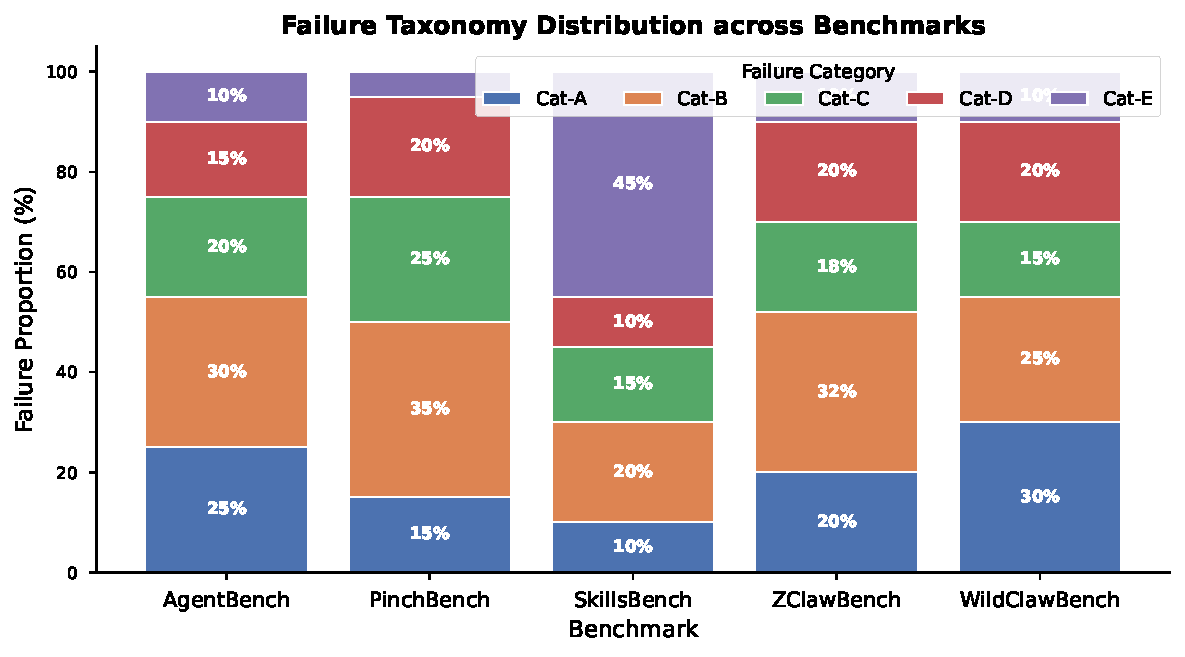
\includegraphics[width=\linewidth]{figs/failure_taxonomy_dist.pdf}
  \caption{Failure category distribution across five agent benchmarks (mock data; to be replaced with annotated results). Category B (Tool/Env Grounding) and C (Memory/State) dominate most benchmarks, while SkillsBench shows a pronounced Category E (Skill Utilization) profile.}
  \label{fig:failure-taxonomy-dist}
\end{figure}
